В данной работе мы анализируем парадигму обучения self-supervised \linebreak learning на примере метода SimCLR \cite{simclr}. Указанный метод сочетает эффективность алгоритмов с контрастной функцией потерь и простоту реализации. Данный раздел посвящен подробному описанию метода SimCLR.

\begin{figure}[H]
    \centering
    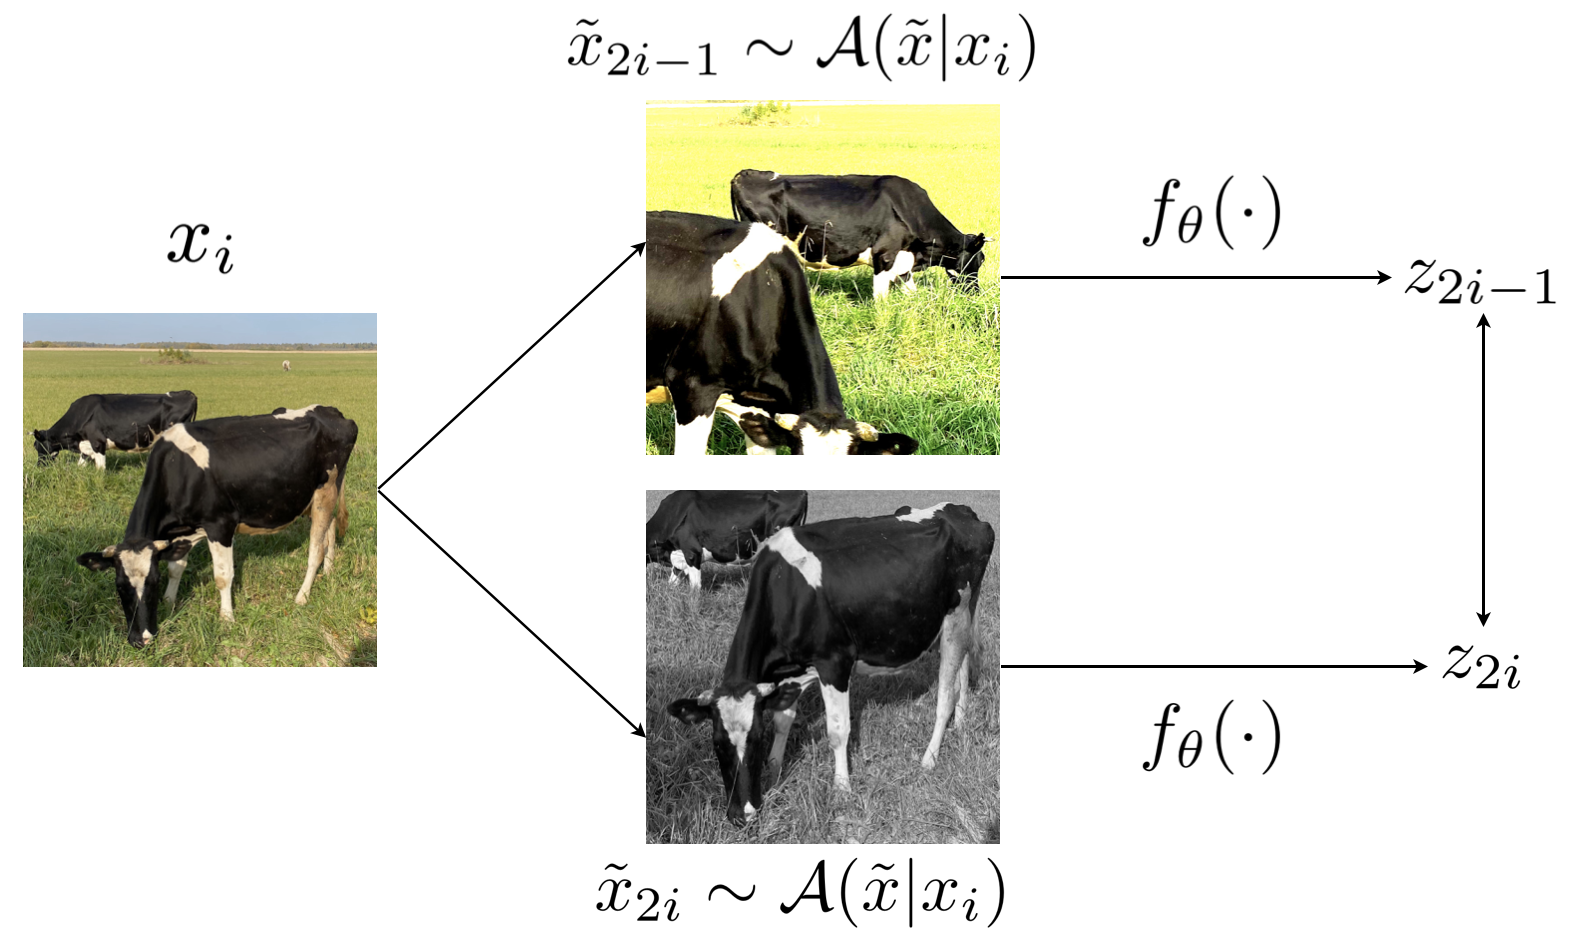
\includegraphics[width=14cm]{images/simclr.png}
    \caption{Схема работы метода SimCLR.}
    \label{simclr:pic:1}
\end{figure}{}

Пусть определена нейронная сеть $f_{\theta}: \R^{H \times W \times C} \rightarrow \R^d$, параметризованная весами $\theta \in \R^{\Theta}$, где $H \times W \times C$ --- размерности изображения, а $d$ --- размерность получаемого векторного представления. Рассмотрим один шаг обучения алгоритма на пакете изображений $\{x_i\}_{i=1}^B, x_i \in \R^{H \times W \times C}$ размера $B$. Пусть опредено некоторое распределение аугментаций $\mathcal{A}(\tilde{x}|x)$, зависящее от изображения $x$. Для каждого изображения $x_i$ из пакета метод генерирует две независимые случайные аугментации $\tilde{x}_{2i-1}, \tilde{x}_{2i} \sim \mathcal{A}(\tilde{x}|x_i)$. Затем данные аугментации пропускаются через нейронную сеть, на выходе получаются представления $z_{2i-1} = f_{\theta}(\tilde{x}_{2i-1})$ и $z_{2i} = f_{\theta}(\tilde{x}_{2i})$; $z_{2i-1}, z_{2i} \in \R^d$ (см. рис. \ref{simclr:pic:1}). Описанная процедура повторяется для всех изображений в пакете, на выходе имеем удвоенный пакет векторных представлений $\{z_{j}\}_{j=1}^B$, каждому изображению $x_i$ соответствуют два представления $z_{2i-1}$ и $z_{2i}$.

Для оптимизации параметров нейронной сети используется контрастная функция потерь \cite{contrastive}. Фактически, перед нейронной сетью ставится задача найти пару для каждого векторного представления. При этом среди всех представлений имеется один позитивный пример (собственно, представление парной аугментации изображения) и $2B-2$ негативных примера (все остальные представления). Определим вероятность $p(z_r|z_i)$ того, что представление $z_r$ соответствует представлению $z_i$:

\begin{equation}
    p(z_r|z_i) = \frac{\exp(\text{sim}(z_r, z_i)/\tau)}{\sum_{k=1}^{2B} [k \ne i] \exp(\text{sim}(z_k, z_i)/\tau)},
\end{equation}

\noindent
где $\text{sim}(u, v)$ --- некоторая функция похожести между векторами $u, v \in \R^d$ (в простейшем случае косинусное расстояние $\text{sim}(u, v) = u^T v /(\|u\|_2 \cdot \|v\|_2)$, $[k \ne i]$ - индикатор, равный 1 при $k \ne i$ и 0 в ином случае, а $\tau > 0$ --- гиперпараметр температуры. По сути, вероятность $p(z_r|z_i)$ задается через оператор softmax на похожестях векторных представлений, что задает дискретное вероятностное распределение на представлениях. Наряду с этим, для каждого представления задан истинный класс ($z_{2k-1}$ для $z_{2k}$ и $z_{2k}$ для $z_{2k-1}$), а остальные $2B-2$ класса являются ложными. Таким образом, метод SimCLR можно рассматривать как классификацию представлений внутри одного пакета, а контрастная функция потерь $\mathcal{L}(\theta, \{x_k\}_{k=1}^B)$ получается эквивалентной кросс-энтропийной функции потерь:
\begin{equation}
    \mathcal{L}(\theta, \{x_k\}_{k=1}^B) = -\frac{1}{2B} \sum_{k=1}^B \Big(\log p(z_{2k}|z_{2k-1}) + \log p(z_{2k-1}|z_{2k})\Big)
\end{equation}

\noindent
Оптимизационный процесс рассчитан на минимизацию мат. ожидания контрастной функции потерь по распределению обучающей выборки $\mathcal{D}$:
\begin{equation}
    \E_{\{x_k\}_{k=1}^B \sim \mathcal{D}} \Big[ \mathcal{L}(\theta, \{x_k\}_{k=1}^B) \Big] \rightarrow \min_{\theta}
\end{equation}
